\documentclass{report}

\input{~/dev/latex/template/preamble.tex}
\input{~/dev/latex/template/macros.tex}

\title{\Huge{}}
\author{\huge{Nathan Warner}}
\date{\huge{}}
\fancyhf{}
\rhead{}
\fancyhead[R]{\itshape Warner} % Left header: Section name
\fancyhead[L]{\itshape\leftmark}  % Right header: Page number
\cfoot{\thepage}
\renewcommand{\headrulewidth}{0pt} % Optional: Removes the header line
%\pagestyle{fancy}
%\fancyhf{}
%\lhead{Warner \thepage}
%\rhead{}
% \lhead{\leftmark}
%\cfoot{\thepage}
%\setborder
% \usepackage[default]{sourcecodepro}
% \usepackage[T1]{fontenc}

% Change the title
\hypersetup{
    pdftitle={Skyscaper Lab}
}

\begin{document}
    % \maketitle
        \begin{titlepage}
       \begin{center}
           \vspace*{1cm}
    
           \textbf{Lab Report 1}
    
           \vspace{0.5cm}
            Skyscaper
                
           \vspace{1.5cm}
    
           \textbf{Nathan Warner}
    
           \vfill
                
                
           \vspace{0.8cm}
         
           
\includegraphics[width=0.4\textwidth]{~/niu/seal.png} \\
           January 30, 2023
           
                
       \end{center}
    \end{titlepage}
    \tableofcontents
    \pagebreak 
    \section{Theory}
    \bigbreak \noindent 
    The objective of this report is to use unit conversion and estimation to find the number of people working in the Willis Tower and to find the water usage of the tower in liters per minute.

    \bigbreak \noindent 
    \section{Data}
    \bigbreak \noindent 
    \begin{center}
        \begin{tabular}{cccc}
            Group \# & Usable Area $(m^{2})$ & Workers & Water Usage $(L/\text{min}) $ \\
            \hline
            1 (My Group)  & 970,000 & 80,000 & 21,000 \\
            2 & 1,500,000 & 100,000 & 25,000 \\
            3 & 2,000,000 & 180,000 & 45,000 \\
            4 & 1,200,000 & 80,000 & 20,000 \\
        \end{tabular}
        \smallbreak \noindent
        \textit{Table 1: Final results from group rounded to two significant figures}
    \end{center}


    \bigbreak \noindent 
    \section{Results}
    \bigbreak \noindent 
    To estimate the number of usable area in the building, we first compute the first floor. If the dimensions are $450ft \times 450ft $, then the area is computed by
    \begin{align*}
        &(450ft)^{2} \\
        =&202500ft^{2}
    .\end{align*}
    \bigbreak \noindent 
    Examing figure 1, we deduce each subregion is given by
    \begin{align*}
        &\frac{202500ft^{2}}{9} =22500ft^{2}
    .\end{align*}
    Takinng the square root gives
    \begin{align*}
        &\sqrt{22500ft^{2}} =150ft
    .\end{align*}
    Thus, each subregion has the dimensions $150ft\ \times\ 150ft$. If we further split each subregion into a 5x5 grid, we get each square (around the perimeter) to be 30ft. With this calculation, we can get good estimations of the unusuable (white space). The calculations for unusable space per subregion is found in the following figure
    \pagebreak \bigbreak \noindent 
    \begin{figure}[ht]
        \centering
        \incfig{figure1}
        \label{fig:figure1}
    \end{figure}
    \begin{center}
        \textit{Figure 1}
    \end{center}

    \bigbreak \noindent 
    Next, we construct classes to represent which floors will have the same area. These findings are summarized in the following table
    \bigbreak \noindent 
    \begin{center}
        \begin{center}
            \begin{tabular}{l|c|c|c}
            Floors & Subregions Available & Unusable area &Usable area \\
            	\hline
            1-49 & All & 55800ft^{2} & $146700ft^{2}$  \\
            50-66 & $R_{1} - R_{8}$ & $78300f^{2}$&  $124200ft^{2}$\\
            67-91 & $R_{4},\ R_{5},\ R_{6},\ R_{9}$& $49500^{2}$ & $40500^{2}$ \\
            92-109 & $R_{5},\ R_{6} $ &$3600ft^{2}$ &$9000ft^{2} $
            \end{tabular}
        \end{center}
    \end{center}
    \bigbreak \noindent 
    Thus, we have the usable area for the entire building
    \begin{align*}
        &49(146700ft^{2}) + 17(124200ft^{2}) + 25(40500ft^{2}) + 18(9000ft^{2}) \\
        =&10474200ft^{2}
    .\end{align*}
    Converting to meters we get
    \begin{align*}
        &10474200ft^{2} \cdot \left(\frac{12in}{1ft}\right)^{2} \cdot \left(\frac{2.54cm}{1in}\right)^{2} \cdot \left(\frac{1m}{100cm}\right)^{2} \\ 
        =&973085.02m^{2}
    .\end{align*}
    Adjusting for two significant figures, we get the total usable area in the building as $970,000m^{2}$
    \bigbreak \noindent 
    Now that we have an estimation for the total usable area, we must estimate how much of this total usable space is actually occupied by cubicles. It may be reasonable to conclude that only $\frac{1}{3}$ of the total usable space is occupied by cubicles. This gives
    \begin{align*}
        &\frac{970000m^{2}}{3} = 320000m^{2}
    .\end{align*}
    \bigbreak \noindent 
    We estimate each cubicle to be $\approx 2m \times 2m = 4m^{2}$. Thus, we have
    \begin{align*}
        &\frac{320000m^{2}}{4m^{2}} = 80000\ \text{cubicles}
    .\end{align*}
    If we deduce that each cubicle can house one person, we have approximately 80,000 workers in the building.
    \bigbreak \noindent 
    Next, we calculate the daily water usage
    \begin{align*}
        &80000\ \text{people} \cdot 100\text{gal} \\
        =&8000000 \text{gal}/\text{day}
    .\end{align*}
    Convering this to liters per minute we get
    \begin{align*}
        &\frac{8000000 \text{ gal}}{\text{1 day}} \times \frac{3.7854 \text{ L}}{1\ \text{gal}}\times \frac{1 \text{ day}}{24\ \text{hours}} \times \frac{1\ \text{hour}}{60 \text{ min}} \\
        =&21000\text{ L}/\text{min}
    .\end{align*}

    \bigbreak \noindent 
    \section{Discussion}
    \bigbreak \noindent 
    Upon reflecting on my report and comparing it with real-world data, it seems I might have been a bit off the mark. The claim from willistower.com about 15,000 people working in the Willis Tower daily makes my estimate of 80,000 workers seem way too high. Furthermore, this estimation also leads to an overestimation of the daily water consumption by the workers. 
    \bigbreak \noindent 
    The dispersion displayed by the table of data is quite interesting. Although the dispersion is quite small, the variation between groups is quite noticable. I believe group four to have findings that are most resonable to real world data.

    \bigbreak \noindent 
    \section{Conclusion}
    \bigbreak \noindent 
    I found it rewarding to enhance my skills in unit conversion and estimation through this exercise. Although it was challenging at the beginning, everything eventually fell into place. In this scenario, we weren't testing a specific theory. It was interesting seeing what other groups were able to estimate. Perhaps more carefully considering how much usable space is actually occupied by cubicles may lead to a more reasonable estimation. 

    \pagebreak 
    \section{Colab Computation}
    \bigbreak \noindent 
    \subsection{Defined Constants}
    \begin{center}
        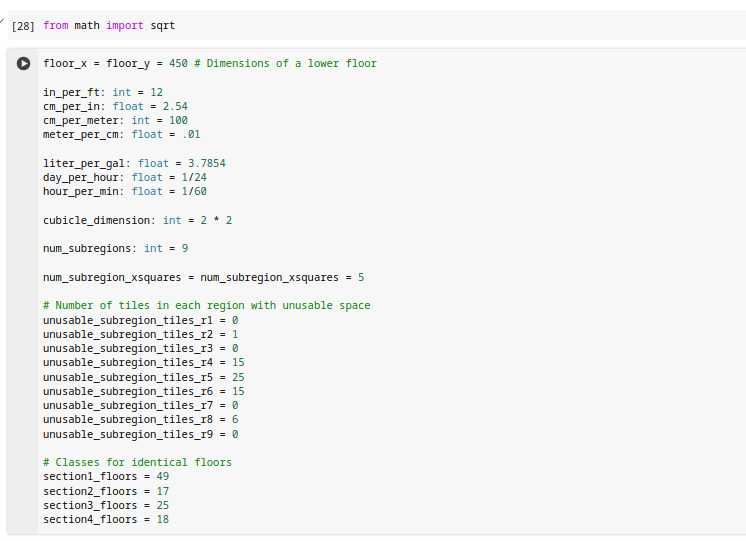
\includegraphics[scale=.5]{./figures/1.png  }
    \end{center}


    \bigbreak \noindent 
    \subsection{Computations}
        \begin{center}
        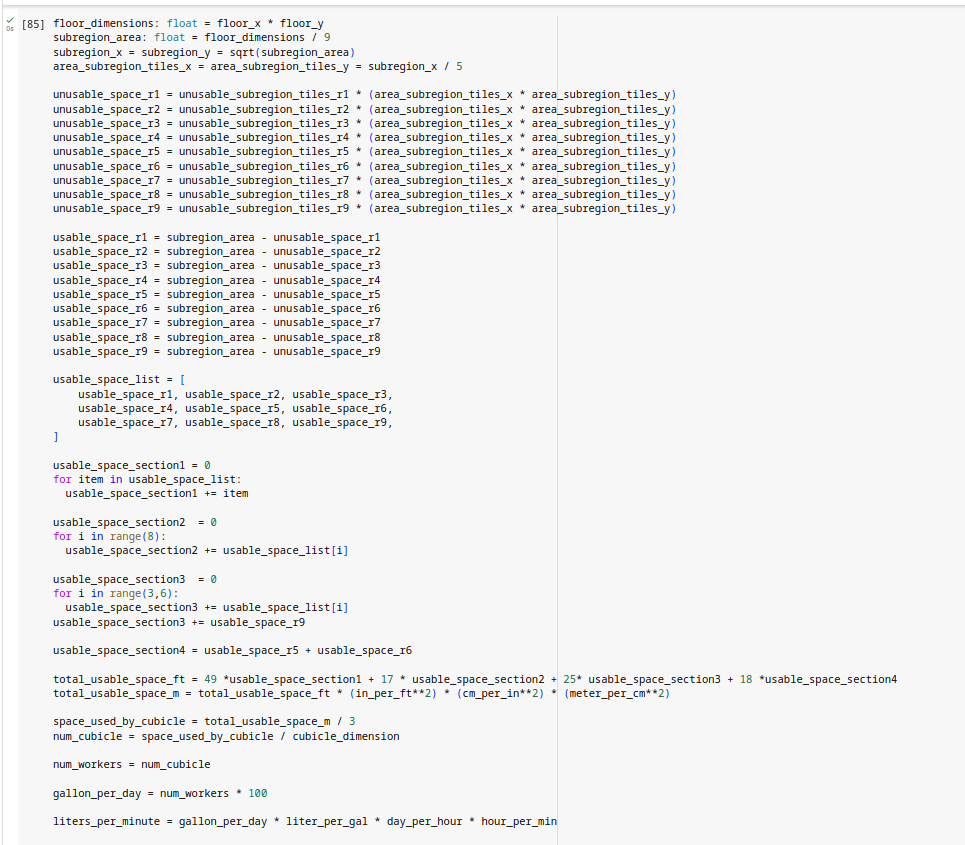
\includegraphics[scale=.5]{./figures/2.png  }
    \end{center}










    
\end{document}
